%! Author = Philipp Emmenegger
%! Date = 09/06/2021

\section{Refactoring}
\textbf{Reasons}
\begin{itemize}
    \item Programs, like people, get old
    \item Broken Windows
    \item Under / Over Engineering
    \item Technical Dept
\end{itemize}

\subsection{Definition}
\begin{itemize}
    \item Systematic approach
    \item Changes are based on a plan
    \item Improve the design of existing code
    \item Retain maintainability of code
    \item Make future changes easier
    \item No new features or functionality
    \item Software works same as before
\end{itemize}

\subsection{Benefits}
\begin{itemize}
    \item Improves the design of software
    \item Makes software easier to understand
    \item Helps to program faster
    \item Helps to find bugs
\end{itemize}

\subsection{Anatomy of a Refactoring}
\textbf{Name}
\begin{itemize}
    \item Builds a common vocabulary
    \item Same idea as giving names to Design Patterns
\end{itemize}
\textbf{Summary}
\begin{itemize}
    \item In which situation do you need it?
    \item What does it do?
\end{itemize}
\textbf{Motivation}
\begin{itemize}
    \item Why the refactoring should be done?
    \item When the refactoring should not be done?
\end{itemize}
\textbf{Mechanics}
\begin{itemize}
    \item How to carry out the refactoring?
    \item Concise, step-by-step description
\end{itemize}
\textbf{Optional sections}
\begin{itemize}
    \item Examples
    \item Inverse refactorings
\end{itemize}
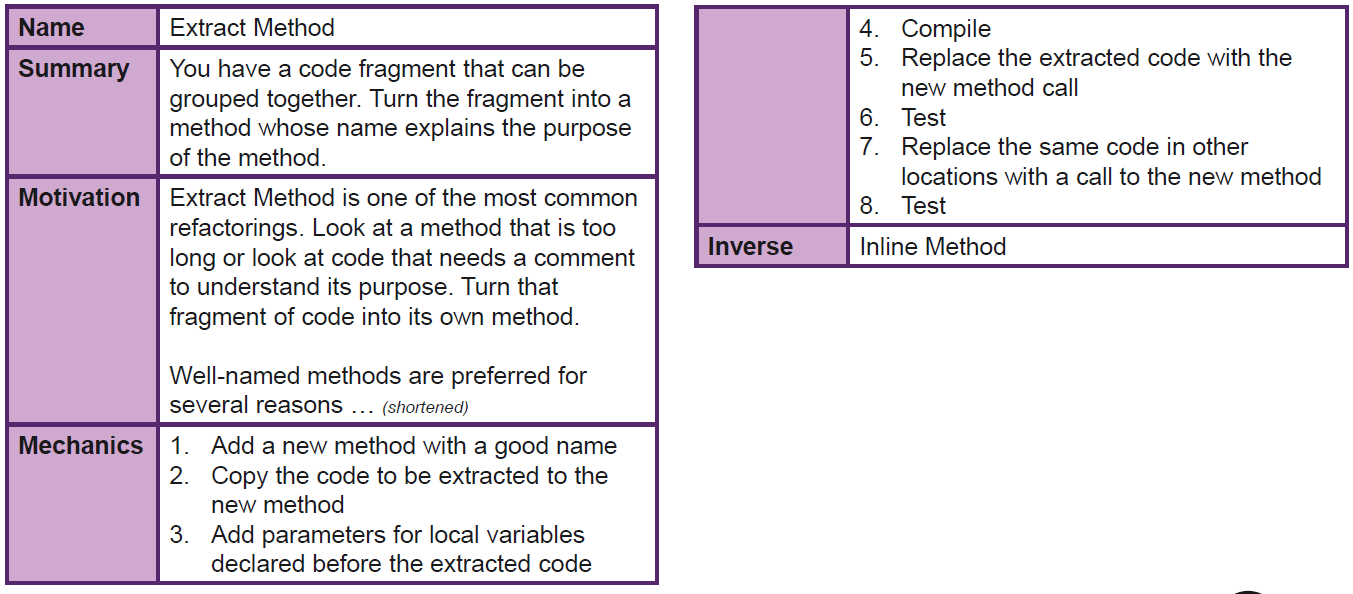
\includegraphics[width=\linewidth]{../img/refactoring_example.png}

\subsection{When to refactor?}
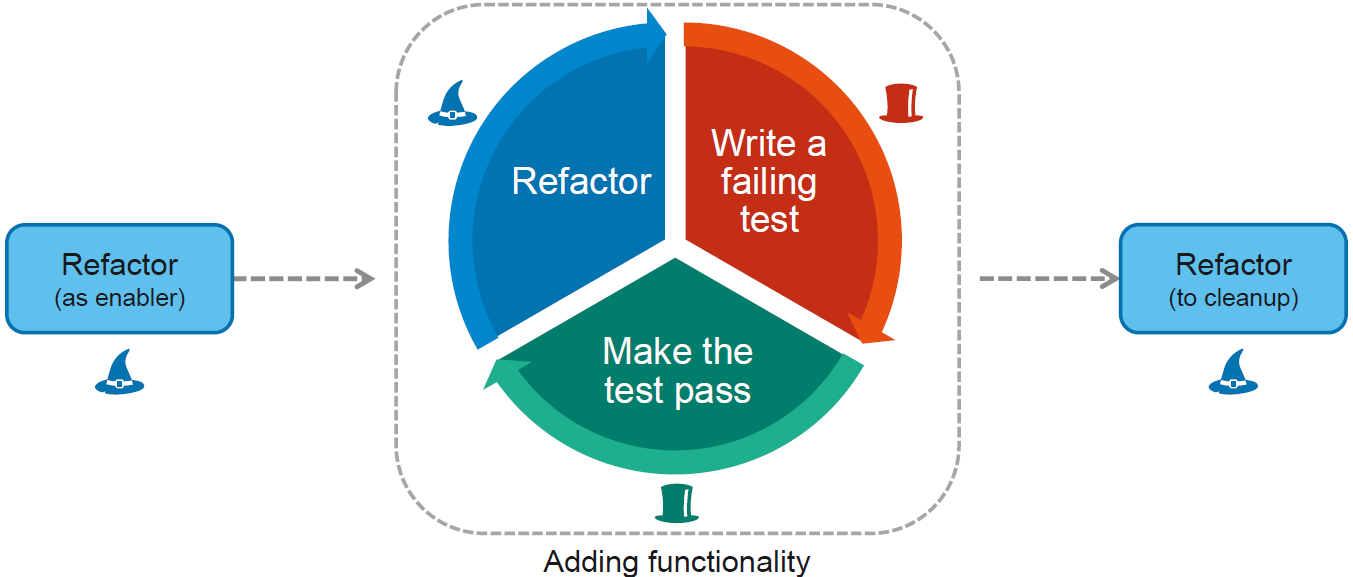
\includegraphics[width=\linewidth]{../img/refactoring_process.png}

\subsection{Code Smells}
\begin{itemize}
    \item Violate properties of Clean Code Principles
    \item Have names
    \item Easy to detect
    \item Have corresponding Refactorings
\end{itemize}
\textbf{Examples:}
\begin{itemize}
    \item Bloaters: Long Method, Large Class, Primitive Obsession..
    \item Object-Orientation Abusers: Switch Statements, Refused Bequest..
    \item Change Preventers: Divergent Change, Shotgun Surgery..
    \item Dispensables: Comments, Duplicated code, Dead Code..
    \item Couplers: Freature Envy, Inappropriate Intimacy..
\end{itemize}

\subsection{Anti Patterns}
\begin{itemize}
    \item Response to recurring problem that is ineffective or contra productive
    \item Have names
\end{itemize}
\textbf{Examples:}
\begin{itemize}
    \item Golden Hammer
    \item Not invented here (Belief that in-house is always better)
    \item Programming by Coincidence
    \item Big ball of mud (no structure)
\end{itemize}

\subsection{Legacy Code}
\begin{itemize}
    \item Valuable code devs are afraid to change
    \item Often lacks automated tests
    \item Contains Dependencies
\end{itemize}
\textbf{Dilemma}\\
When we change code, we should have tests in place. 
To put tests in place, we often have to change code.\\
\textbf{Dependencies}\\
One of the most critical problems in software development.\\
Much legacy code work involves breaking dependencies so that change can be easier.\\
\begin{itemize}
    \item 
\end{itemize}

\subsubsection{Legacy Code Change Algorithm}
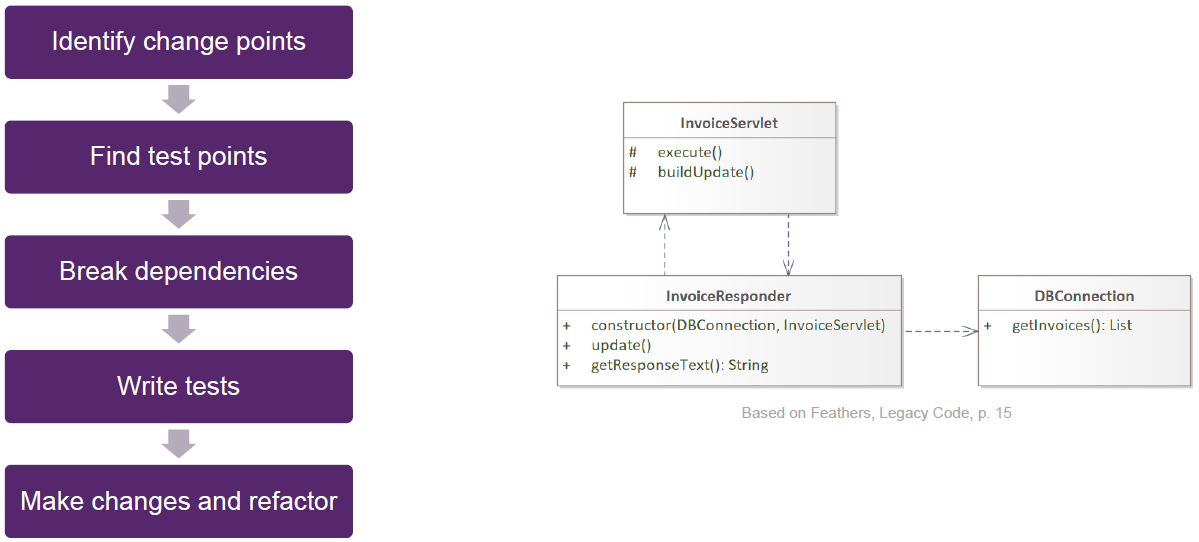
\includegraphics[width=\linewidth]{../img/legacy_code_change_algo.png}
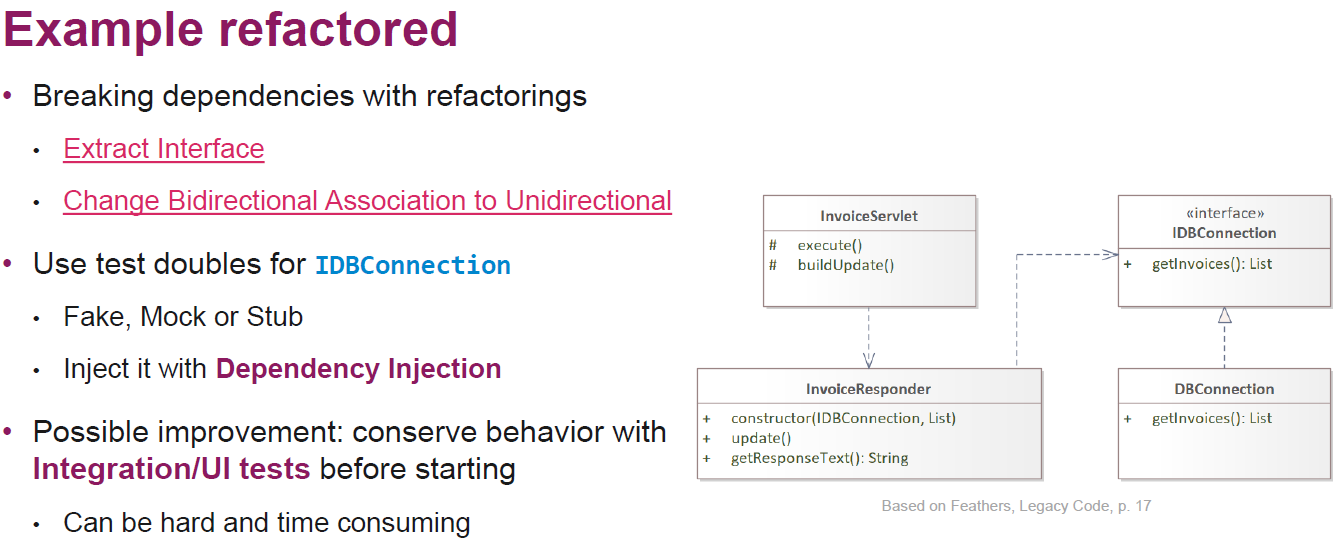
\includegraphics[width=\linewidth]{../img/legacy_code_change_algo_refactored.png}

\subsubsection{Extract and Override - Factory Method}
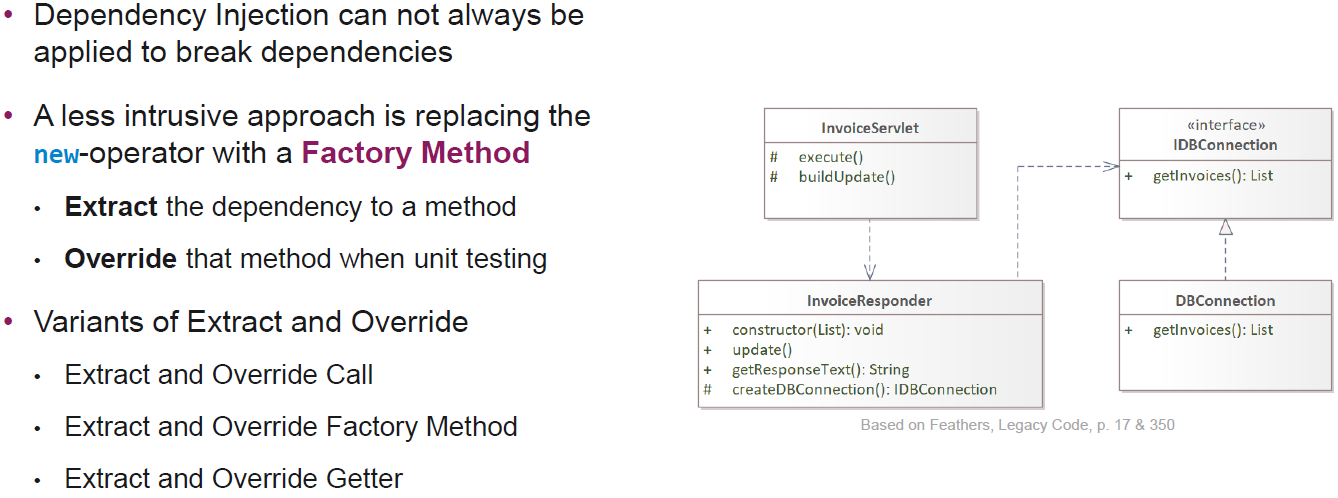
\includegraphics[width=\linewidth]{../img/extract_and_override.png}

\subsubsection{The Gilded Rose Kata}
\begin{enumerate}
    \item Understand the functionality
    \begin{itemize}
        \item Look out for Code Smells
        \item Gather ideas for a clean implementation
    \end{itemize}
    \item Preserve functionality with integration tests
    \item Refactor the existing code
    \item Implement new functionality (TDD Cycle)
\end{enumerate}